
\section{Authenticator}
A authenticator is a software that generates a token that is used with a password when logging in. One possible implementation is generated the token with a seed that is set when created, and a time variable. When we need a token, we concatenate the seed with the timestamp, and then hash it. The first N chars of the hash result are the authenticator token. The server knows the seed, and can generate the same token using the same process. The server is sure that only somebody that knows the seed can generate a valid token.

\subsection{Exercises}
\begin{enumerate}
	\item Write a little program that every second in the UNIX time that ends with 0 prints the token with a given seed. You can use the \textbf{setInterval()} function. Use a SHA256 like in the hash exercise. You can get the UNIX time the following way:
	\begin{lstlisting}[style=JavaScript]
	timestamp = Math.round((new Date()).getTime() / 1000);
	\end{lstlisting}
	\item Write a program that has a bare socket server. If the server receives a valid token, responds "ok!" 
\end{enumerate}


\section{Crypto Proxy}
This exercice proposes the creation of a crypto proxy. To connect to a server we would usually create a raw tcp socket and send information through it. 

We are going to implement a TCP proxy that acts in between the sockets, and encrypts the information passed through it.

\begin{figure}[htb]
	\begin{centering}
		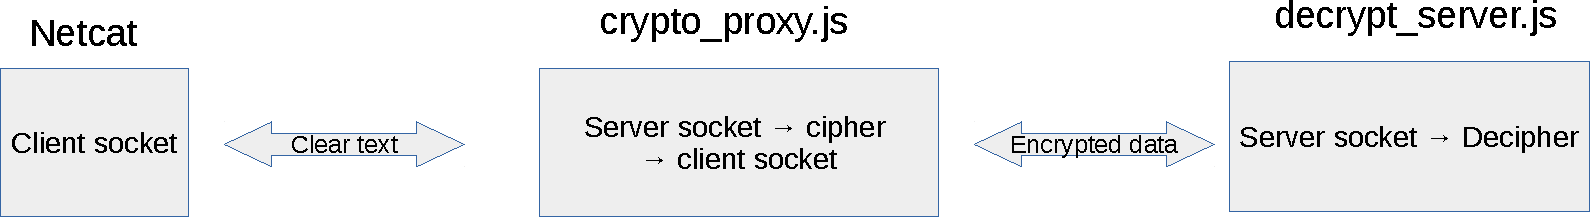
\includegraphics[width=0.7\columnwidth]{\securitydir/basicJsCrypto/figures/crypto_proxy}
		\par\end{centering}
	\caption{\label{fig:crypto_proxy} Connexion scheme}
\end{figure}


For the first socket (local socket), we are going to use netcat. netcat allows to create a TCP socket easily from the CLI. In the real world, netcat would be much more complex program.

The second socket will recieve the unencrypted data, cipher it using AES 256 and resend it to the server.

Finally, the remote socket recieves the encrypted data, and deciphers it. In our implementation, the server saves the data into a file.

To run the experiment we are going to need three different terminals.

\begin{lstlisting}
$ nodejs decrypt_server.js
$ nodejs crypto_proxy.js
$ nc localhost 1234
\end{lstlisting}


If we use wireshark we can see that the first connection is in clear text, while the second isnt.

For the next part, we are going to send a picture through the proxy. To do this, execute netcat with a pipe where Tux.png is the picture to send.

\begin{lstlisting}
$ cat Tux.png | nc localhost 1234
\end{lstlisting}

If all goes well, we shall see a picture named test.png, that should be the same as Tux.png

If we capture this traffic with wireshark, then select the option "Follow TCP Stream" on any tcp packet, and finally select "Save as..." we can capture files directly from wireshark. If we do this with the connection that isn't encrypted, we can save the picture, while if we do this in the connection that isn't, we are getting pseudonoise. This is a very powerful tool, as we can see and save any non-encrypted traffic that goes trough our computer (Now imagine you are the gateway in a public wifi).

\subsection{Exercises}
\begin{enumerate}
	\item Write the decrypt server. It must receive the data from the socket, pipe it through a AES decipher and then save it to a file.
	
	\item Write the proxy server. It should have two different sockets. One that works as a server en receives the data from the netcat, and the other must be a client that connects to the decrypt\_server. The data received from the netcat should be encrypted and then sent to the decrypt server.
	
	\item Improve the proxy and the server so full duplex encrypted conection is possible.
\end{enumerate}

 

\section{Crypto socket with authentication}

In this exercise we are implementing all we've seen until now. We are going to implement a socket that uses both symmetric and asymmetric cryptography. Once the key exchange is done and the connection is fully encrypted, then we're gonna do a user and password login, with a authenticator token.

\begin{figure}[htb]
	\begin{centering}
		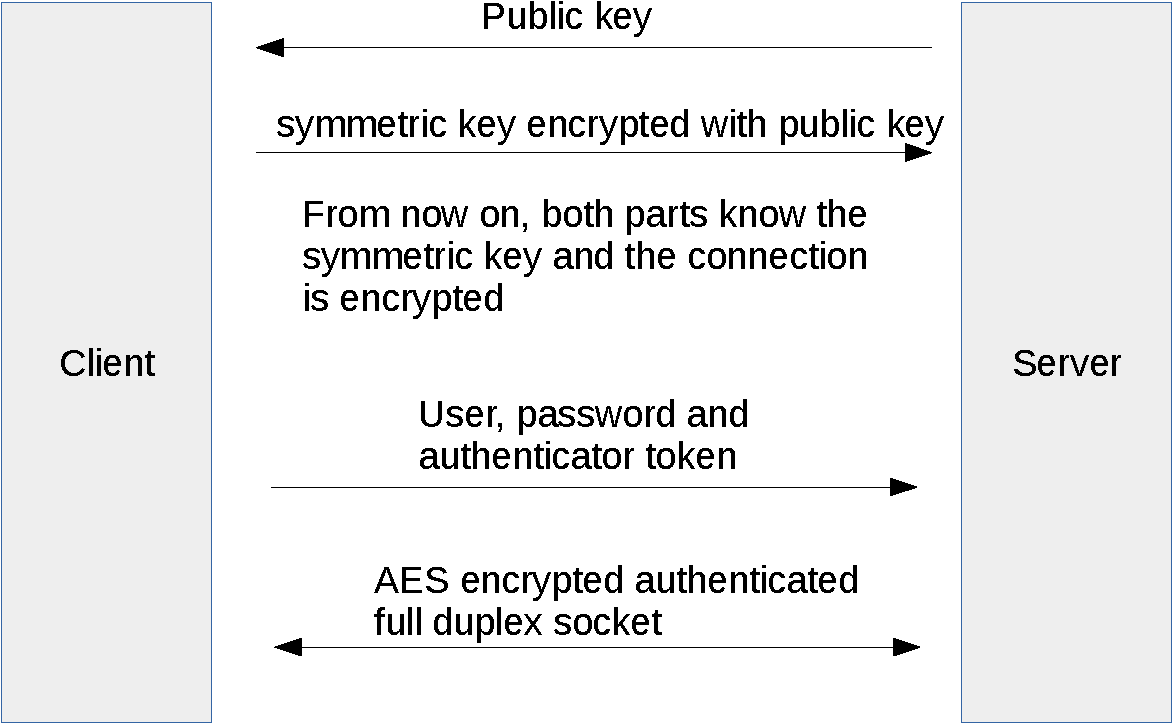
\includegraphics[width=0.7\columnwidth]{\securitydir/basicJsCrypto/figures/authenticated_socket}
		\par\end{centering}
	\caption{\label{fig:authenticated_socket} Connexion scheme}
\end{figure}


\subsection{Exercises}
This software is going to have three parts: client, server and authenticator. The authenticator can be recycled from the previous exercise. 
\begin{enumerate}
	\item First of all design the key exchange. The server should be listening for connections, and on connection send it's public key to the client. The client saves this key, and sends the symmetric key that is going to be used, encrypted with the server's public key, so eavesdropper's can't see it. From this point, both parties have the symmetric key, and all data exchange is gonna be encrypted with this key.
	
	\item Once the private connection is established, develop a login system. The easiest way is to achieve this is to make the client prompt the user with the user, password and authenticator token. Then the client serializes the answer in a JSON object, sends it to the server, and the server deserializes and reads the information. Server must generate a pseudo - DB at startup with a entry for every user that contains their password stored with a bcrypt hash and the seed for the user's authenticator.
	
	Beware that AES won't send the JSON unless it's larger than the block size, so to be sure we'll add a padding consistent of empty spaces.
	
	\begin{lstlisting}[style=JavaScript]
	cipher.write(serialized + " ".repeat(128 - serialized.length));
	\end{lstlisting}
\end{enumerate}


